\documentclass[border=4pt]{standalone}
\usepackage{tikz}
\usepackage{pgfplots}
\pgfplotsset{compat=1.18}
\usetikzlibrary{shapes.geometric,arrows.meta,positioning,calc,fit,decorations.pathreplacing,backgrounds}
\definecolor{boxblue}{RGB}{225,238,252}
\definecolor{boxgreen}{RGB}{225,247,231}
\definecolor{boxorange}{RGB}{253,236,216}
\definecolor{boxgray}{RGB}{237,237,237}
\definecolor{boxred}{RGB}{253,226,226}
\begin{document}
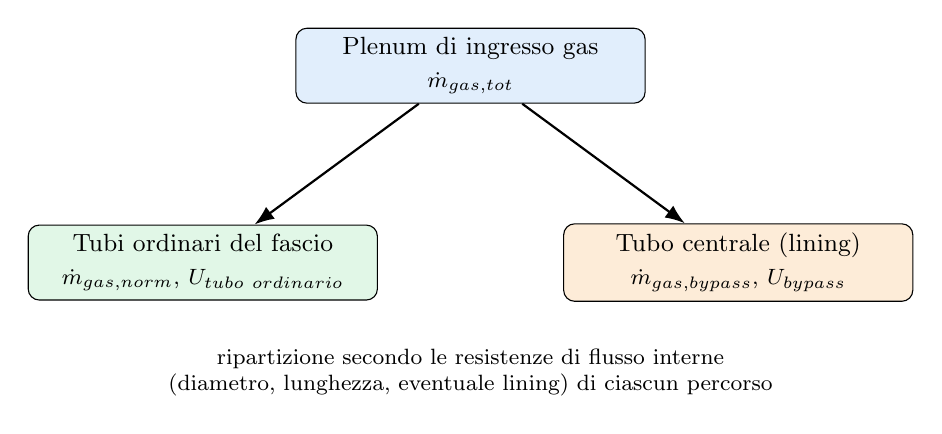
\begin{tikzpicture}[
  box/.style={draw, rectangle, rounded corners, minimum height=0.9cm, text width=4.2cm, align=center, font=\small},
  arr/.style={-{Latex[length=2.5mm]}, thick}
]
\node[box, fill=boxblue] (src) at (0,1.5) {Plenum di ingresso gas\\[1pt]\footnotesize $\dot m_{gas,tot}$};
\node[box, fill=boxgreen] (b1) at (-3.4,-1.0) {Tubi ordinari del fascio\\[1pt]\footnotesize $\dot m_{gas,norm}$, $U_{tubo\ ordinario}$};
\node[box, fill=boxorange] (b2) at (3.4,-1.0) {Tubo centrale (lining)\\[1pt]\footnotesize $\dot m_{gas,bypass}$, $U_{bypass}$};
\node[font=\footnotesize,align=center] at (0,-2.4) {ripartizione secondo le resistenze di flusso interne\\ (diametro, lunghezza, eventuale lining) di ciascun percorso};

\draw[arr] (src) -- (b1);
\draw[arr] (src) -- (b2);
\end{tikzpicture}
\end{document}
